\documentclass[11pt]{amsbook}

\usepackage{../HBSuerDemir}	% ------------------------

\begin{document}

% ++++++++++++++++++++++++++++++++++++++
\hPage{b2p2/339}
% ++++++++++++++++++++++++++++++++++++++

\begin{hEnumerateArabic}
	
	\item
	Let $q_{1}, \cdots , q_{n}$ be $n$ values of $q=f(x)$ for n direct measurements of $x_{1}, \cdots , x_{n}$, where $f$ is known function. In this case $q_{i}$'s become \hDefined{indirect} measurements of $q$.
	
	It can be shown that the best value $\bar q$ of $q$ is $\bar q = f(\bar x)$ where $\bar x$ and $\bar y$ are the arithmetic means of $x_{i}$'s and $q_{i}$'s respectively.
	\begin{exmp}
		The length $l$ of a simple pendulum is measured as 24,8; 25,1; 25,0; 24,8; 25,0; 25,1; 24,7; 25,1 cm. Then
		\begin{hEnumerateAlpha}
		
			\item
			find the best length $\bar l$
			
			\item
			find the best period.
		\end{hEnumerateAlpha}
		
		\begin{hSolution}
			\begin{hEnumerateAlpha}
			
				\item
				$\bar l = ( \sum l_{i})/8 = 24,95$ cm,
				
				\item
				$ T = \pi \sqrt{l / g} = \pi \sqrt{24,95/g} = 4.99\pi / \sqrt{g}$.
			\end{hEnumerateAlpha}
		\end{hSolution}
	\end{exmp}
	
	\item
	Let $y$ be related  to $x$ by an unknown function $f$, and let $y_{1}, \cdots , y_{n}$ be the measured values of y corresponding to a set of selected values $x_{1}, \cdots , x_{n}$ of $x$.
	
	\begin{multicols}{2}
		When one plots the points $P_{i} ( x_{i}, y_{i})$ on a rectangular coordinate system 0xy, we obtain a distribution of y against x.

		Now the problem is to determine the best function giving this distribution.
	
		The solution of the problem involves the following steps:
		
		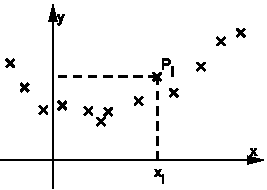
\includegraphics[width=0.4\textwidth]{images/b2p2-339-fig01}
	\end{multicols}
	
	\begin{hEnumerateRoman}
	
		\item
		from the distribution guess the type of the function as linear,quadratic, exponential, $\cdots$ ,
		
		\item
		write the general form of the function,
		
		\item
		by the use of the MLS, determine the unknown parameters.
	\end{hEnumerateRoman}
\end{hEnumerateArabic}


% =======================================================
\end{document}  